\documentclass{article}
\usepackage{amsmath}
\usepackage{amssymb}
\newcommand*{\qed}{\hfill\ensuremath{\blacksquare}}
\usepackage{graphicx}
\graphicspath{{.}}
\usepackage{hyperref}
\usepackage{tikz}
\usepackage{pgfplots}
\long\def\/*#1*/{}
\usetikzlibrary{arrows}


\title{Computational Linear Algebra, Module 11}
\author{Maya Shende}
\date{Due: April 18th, 2018}

\begin{document}
\maketitle

\begin{enumerate}

%exercise 1
\item $AS = A
\begin{bmatrix}
\vdots	&\vdots	&\dots	&\vdots\\
x_1	&x_2		&\ddots	&x_n\\
\vdots	&\vdots	&\dots	&\vdots
\end{bmatrix}
=
\begin{bmatrix}
\vdots	&\vdots	&\dots	&\vdots\\
Ax_1		&Ax_2	&\ddots	&Ax_n\\
\vdots	&\vdots	&\dots	&\vdots
\end{bmatrix}
=
\begin{bmatrix}
\vdots	&\vdots	&\dots	&\vdots\\
\lambda x_1		&\lambda x_2	&\ddots	&\lambda x_n\\
\vdots	&\vdots	&\dots	&\vdots
\end{bmatrix}
$. Now, $\Lambda = 
\begin{bmatrix}
\lambda_1		&0	&\dots	&\dots\\
0	&\lambda_2	&\dots	&\dots\\
\vdots	&\vdots	&\ddots	&\dots\\
\vdots	&\vdots	&\dots	&\lambda_n
\end{bmatrix}
$. So, \\$S\Lambda = 
\begin{bmatrix}
\vdots	&\vdots	&\dots	&\vdots\\
x_1	&x_2		&\ddots	&x_n\\
\vdots	&\vdots	&\dots	&\vdots
\end{bmatrix}
\begin{bmatrix}
\lambda_1		&0	&\dots	&\dots\\
0	&\lambda_2	&\dots	&\dots\\
\vdots	&\vdots	&\ddots	&\dots\\
\vdots	&\vdots	&\dots	&\lambda_n
\end{bmatrix}
=
\begin{bmatrix}
\vdots	&\vdots	&\dots	&\vdots\\
\lambda x_1		&\lambda x_2	&\ddots	&\lambda x_n\\
\vdots	&\vdots	&\dots	&\vdots
\end{bmatrix}
$\qed\\
However, $AS \neq \Lambda S$ because when you change the order, the $\lambda$'s would distribute into the rows of $S$ instead of the columns. 
%exercise 2
\item The dimensions of \textbf{C} is $m \times n$ or $3 \times 4$. \\
	Example:
	$$ \textbf{A} = \begin{bmatrix} 2 \\ 4 \\ 6 \end{bmatrix} \text{ and } \textbf{B} = \begin{bmatrix} 1 & 3 & 5 & 7 \end{bmatrix}$$
	Therefore, $\textbf{AB} = \textbf{C}$ is:
	$$ \textbf{C} = \begin{bmatrix} 2 \\ 4 \\ 6 \end{bmatrix} \begin{bmatrix} 1 & 3 & 5 & 7 \end{bmatrix} = 
	\begin{bmatrix} 
	2 & 6 & 10 & 14  \\ 
	4 & 12 & 20 & 28  \\
	6 & 18 & 30 & 42  
	\end{bmatrix}$$

%exercise 3
\item $a_4 = 
\begin{bmatrix}
1	&1	&1	&1
\end{bmatrix}
$, so, $a_4a_4^T + 2a_4a_4^T + 3a_4a_4^T = \\
\begin{bmatrix}
1	&1	&1	&1
\end{bmatrix}
\begin{bmatrix}
1\\
1\\
1\\
1
\end{bmatrix}
+ 2
\begin{bmatrix}
1	&1	&1	&1
\end{bmatrix}
\begin{bmatrix}
1\\
1\\
1\\
1
\end{bmatrix}
+ 3
\begin{bmatrix}
1	&1	&1	&1
\end{bmatrix}
\begin{bmatrix}
1\\
1\\
1\\
1
\end{bmatrix}
= \\
\begin{bmatrix}
1	&1	&1	&1\\
1	&1	&1	&1\\
1	&1	&1	&1\\
1	&1	&1	&1
\end{bmatrix}
+ 
\begin{bmatrix}
2	&2	&2	&2\\
2	&2	&2	&2\\
2	&2	&2	&2\\
2	&2	&2	&2
\end{bmatrix}
+ 
\begin{bmatrix}
3	&3	&3	&3\\
3	&3	&3	&3\\
3	&3	&3	&3\\
3	&3	&3	&3
\end{bmatrix}
= 
\begin{bmatrix}
6	&6	&6	&6\\
6	&6	&6	&6\\
6	&6	&6	&6\\
6	&6	&6	&6
\end{bmatrix}
$
%exercise 4
\item Let $A = 
\begin{bmatrix}
1	&3	&2\\
2	&1	&3
\end{bmatrix}
$ and $B = 
\begin{bmatrix}
1	&2	&3	&1\\
2	&3	&2	&2\\
3	&1	&1	&3
\end{bmatrix}
$. Then, $AB = 
\begin{bmatrix}
13	&13	&10	&13\\
13	&10	&11	&13
\end{bmatrix}
$. Now for the right hand side, we have \\$\sum_{i=1}^{k} a_ib_i^T = 
\begin{bmatrix}
1\\
2
\end{bmatrix}
\begin{bmatrix}
1	&2	&3	&1
\end{bmatrix}
+
\begin{bmatrix}
3\\
1
\end{bmatrix}
\begin{bmatrix}
2	&3	&2	&2
\end{bmatrix}
+
\begin{bmatrix}
2\\
3
\end{bmatrix}
\begin{bmatrix}
3	&1	&1	&3
\end{bmatrix}
 = \\
 \begin{bmatrix}
 1	&2	&3	&1\\
 2	&4	&6	&2
 \end{bmatrix}
 +
 \begin{bmatrix}
 6	&9	&6	&6\\
 2	&3	&2	&2
 \end{bmatrix}
 +
 \begin{bmatrix}
 6	&2	&2	&6\\
 9	&3	&3	&9
 \end{bmatrix}
 = 
 \begin{bmatrix}
13	&13	&10	&13\\
13	&10	&11	&13
\end{bmatrix}
$. 
%exercise 5
\item 

%exercise 6
\item 	
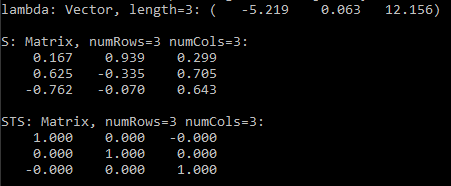
\includegraphics[scale=1]{exercise6}
	\\\\
	The columns of \textbf{S} are orthogonal.

%exercise 7
\item Example matrix: $
\begin{bmatrix}
\frac{1}{2}	&1	&\frac{1}{2}\\
1	&2	&1\\
\frac{1}{2}	&1	&\frac{1}{2}
\end{bmatrix}
$ and the associated eigenvalues and eigenvectors output are:\\

\includegraphics[scale=0.7]{exercise7}

%exercise 8
\item $A = 
\begin{bmatrix}
r_1	&r_2	&\dots	&r_n\\
\vdots	&\vdots	&\ddots	&\vdots\\
\dots	&\dots	&\dots	&\dots	
\end{bmatrix}
$ and $B = 
\begin{bmatrix}
b_{11}	&b_{12}	&\dots	&b_{1k}\\
\vdots	&\vdots	&\ddots	&\vdots\\
b_{n1}	&b_{n2}	&\dots	&b_{nk}
\end{bmatrix}
$ so $C = 
\begin{bmatrix}
r_1b_{11} + r_2b_{21} + \dots + r_nb_{n1}	&\dots	&r_1b_{1k} + r_2b_{2k} + \dots r_nb_{nk}\\
\vdots	&\vdots	&\ddots	&\vdots\\
\dots	&\dots	&\dots	&\dots
\end{bmatrix}
$. So, as we can see from this, the first element of $C$ is a linear combination of the first column of $B$, the second element of $C$ is a linear combination of the second column of $B$ and so on. So, we can say that the whole first row of $C$ is a linear combination of the rows of $B$. 

%exercise 9
\item $A = 
\begin{bmatrix}
r_1	&r_2	&\dots	&r_n\\
\vdots	&\vdots	&\ddots	&\vdots\\
\dots	&\dots	&\dots	&\dots	
\end{bmatrix}
$ and $B = 
\begin{bmatrix}
b_{11}	&b_{12}	&\dots	&b_{1k}\\
\vdots	&\vdots	&\ddots	&\vdots\\
b_{n1}	&b_{n2}	&\dots	&b_{nk}
\end{bmatrix}
$. So, \\
$C = 
\begin{bmatrix}
r_1b_{11} + r_2b_{21} + \dots + r_nb_{n1}	&\dots	&r_1b_{1k} + r_2b_{2k} + \dots r_nb_{nk}\\
a_{21}b_{11} + a_{22}b_{21} + \dots + a_{2n}b_{n1}	&\dots	&a_{21}b_{1k} + a_{22}b_{2k} + \dots a_{2n}b_{nk}\\
\vdots		&\ddots	&\vdots\\
a_{m1}b_{11} + a_{m2}b_{21} + \dots + a_{mn}b_{n1}	&\dots	&a_{m1}b_{1k} + a_{m2}b_{2k} + \dots a_{mn}b_{nk}
\end{bmatrix}
$. So, we can see that each element in the first column of $C$ is a linear combination of each row of $A$. So, we can say that the whole first column of $C$ is a linear combination of all of the columns of $A$. 

%exercise 10
\item Eigenvalue, eigenvector pairs correspond to the amount of change in each dimension of the space we are working with. A space consists of the linearly independent components, or the span, and we know that the $rank(A)$ is the number of linearly independent dimensions of the space represented by A. Thus, the $rank(A) = rank(\Lambda) = $ number of nonzero eigenvalues. 

%exercise 11
\item When we multiply $z^T$ by $x_i$, we are going to do $x_i$ with every term in $z^T$. Since the $x_i$'s are orthogonal, $x_i \cdot x_i = 1$ and $x_i \cdot x_j = 0, i \neq j$. So, the only term that will remain is going to be $\alpha_i$, and all terms will go to zero. 

%exercise 12
\item We want to show that $A^TA$ is positive definite for any matrix $A$. So, we need to show that $z^TA^TAz > 0$. So, \\
$z^TA^TAz = (Az)^T(Az) = (Az)\cdot(Az) \geq 0$, and when $A$ is non-singular, this dot product is strictly greater than 0. So, $A^TA$ is positive definite. \qed

%exercise 13
\item plot for DataExample.java: \\
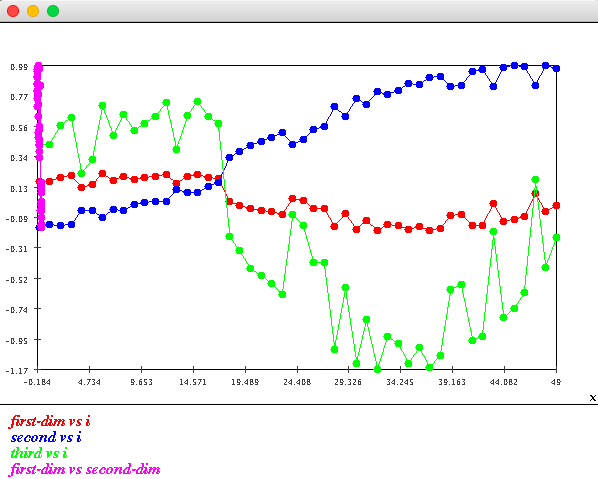
\includegraphics[scale=0.3]{exercise13_original}\\
It does not look like adding the plot of one dimension agains another helps here. \\
The dimension of the PCA coordinates being plotted is the first dimension:\\
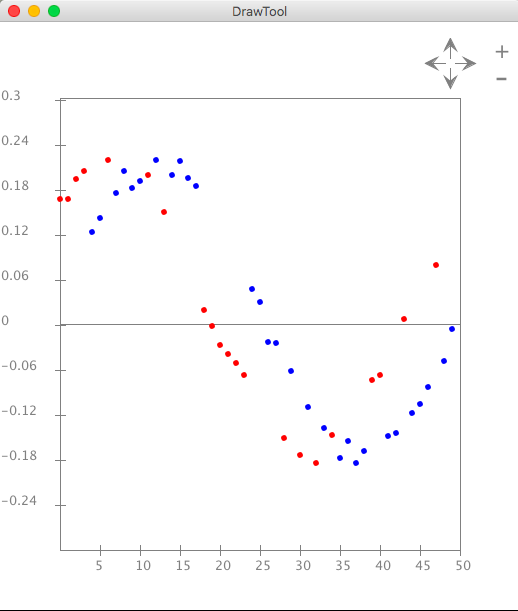
\includegraphics[scale=0.3]{exercise13_pca}

%exercise 14
\item We first normalize the data so that the mean is 0 (center the data). Then we compute the covariance matrix and actually find the eigenvectors of this matrix. 

%exercise 15
\item Mean Vector = $\begin{bmatrix}1.5\\3\\0\end{bmatrix}$

%exercise 16
\item Mean Vector = $\begin{bmatrix}1.5\\3\\0\end{bmatrix}$\\
	Mean of the Mean Vector = $\begin{bmatrix}0\\0\\0\end{bmatrix}$

%exercise 17
\item Covariance Matrix: \\
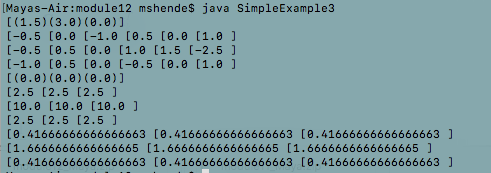
\includegraphics[scale=0.5]{exercise17}

%exercise 18
\item Based on Useful Fact \#1, we know that if $\textbf{C} = \textbf{AB}$ then $\textbf{c}_i = \textbf{A}\textbf{b}_i$ for all columns in both $\textbf{C}$ and $\textbf{B}$. Using this fact, we can look at each individual column in both $\textbf{S}$ and ${\bf \Lambda}$ and perform the products of them in the desired order. With the resulting vectors, we can re-compile them into a covariance matrix.

%exercise 19
\item DataExample3.java: \\
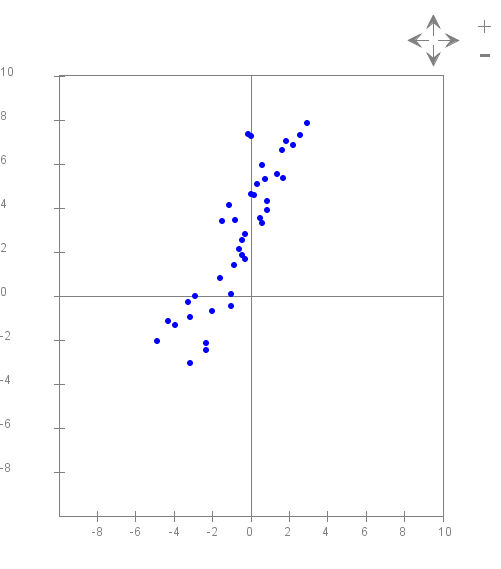
\includegraphics[scale=0.3]{exercise19_1}\\
PCAExample2.java: \\
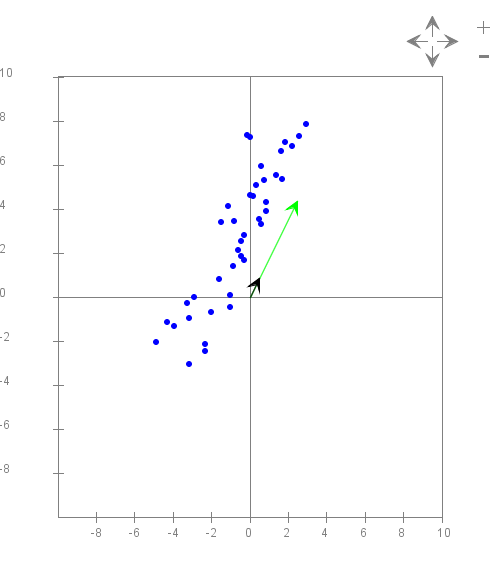
\includegraphics[scale=0.3]{exercise19_2}

%exercise 20
\item If we use useful fact 1, we can treat $S^T$ as $A$ and $X$ as $B$, and then distribute the columns in reverse to see that $Y=S^TX$ follows from $y_i = S^Tx_i$. 

%exercise21
\item First, if we let $z=(1, 1, 1, \dots, 1)$ and $X$ be a centered data matrix, then when we multiply $Xz$, we see that for each row of $X$, the values will just sum to 0 (since they are centered evenly using their mean about 0). So, we will get $Xz = 0$. Now, we want to show that $Yz = 0$. So, substituting $Y = BX$, we have $BXz = B0 = 0$. Therefore, we have shown that $Yz = 0$ and thus $Y$ is centered. 

%exercise22
\item The same pattern is observed:\\
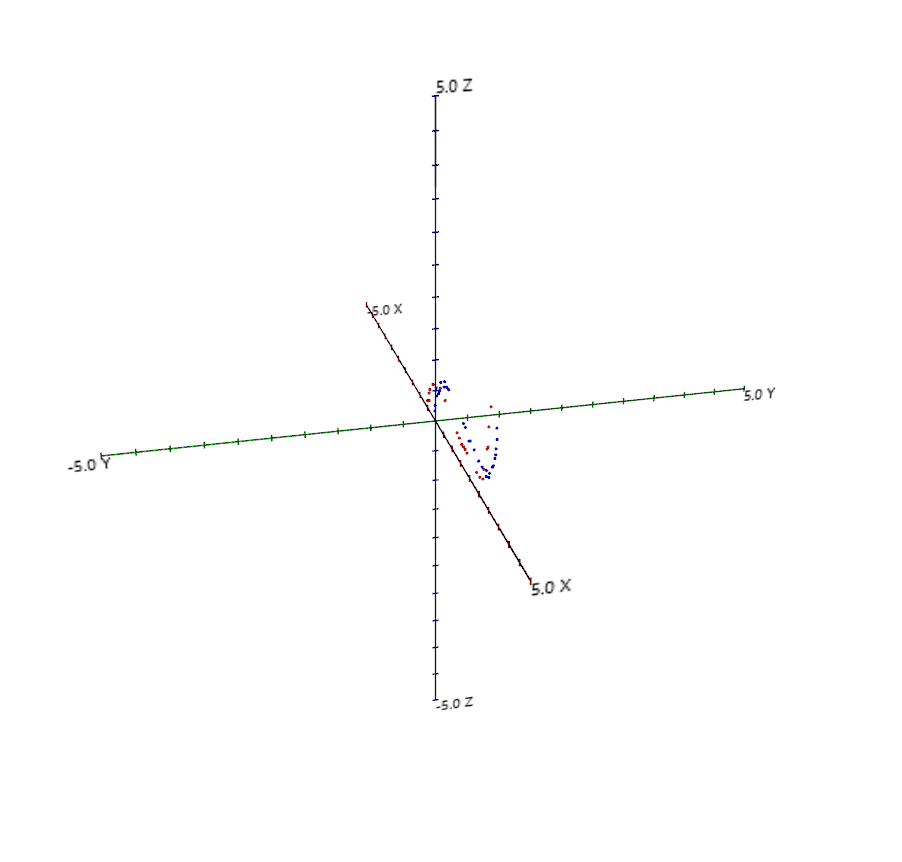
\includegraphics[scale=0.3]{exercise22}

%exercise 23
\item Two Applications of Clustering:
	\begin{enumerate}
		\item Targeting Marketing Programs: group people with similar interests together and advertise the same thing to them.
		\item Land Usage: Similar plots of land can be used for the same thing. 
	\end{enumerate}
	
%exercise 24
\item DataExample3.java:\\
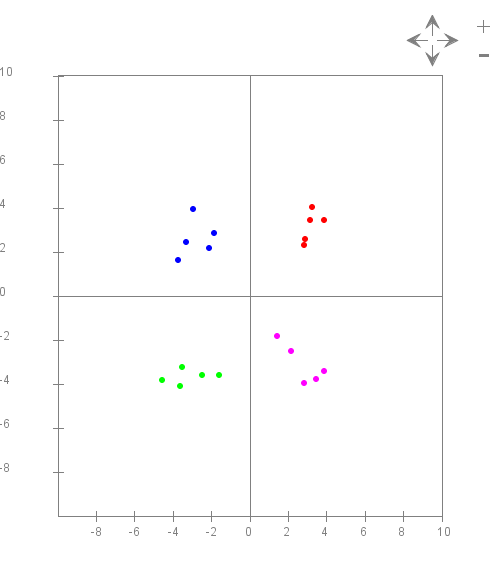
\includegraphics[scale=0.45]{exercise24_1}\\
PCAExample3.java:\\
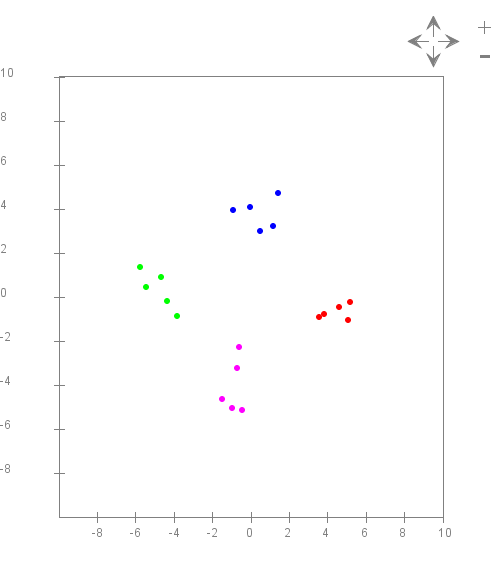
\includegraphics[scale=0.45]{exercise24_2}

%exercise25
\item Hyperplanes would not work because the data is not clustered into non-overlapping areas. Instead the data is formatted with one type being in the middle and another going around the outside. The K-means algorithm will assign the center of the blue data points and the red data points at the same spot and the planes would overlap. \\
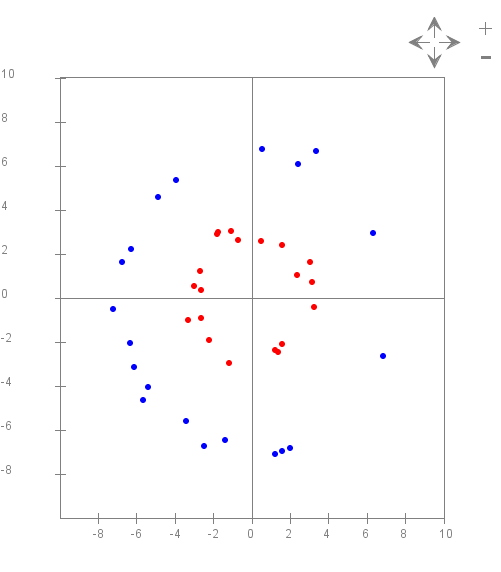
\includegraphics[scale=0.45]{exercise25}

%exercise26
\item The PCA-transformed points are not easier to cluster because they are tightly mixed together. \\
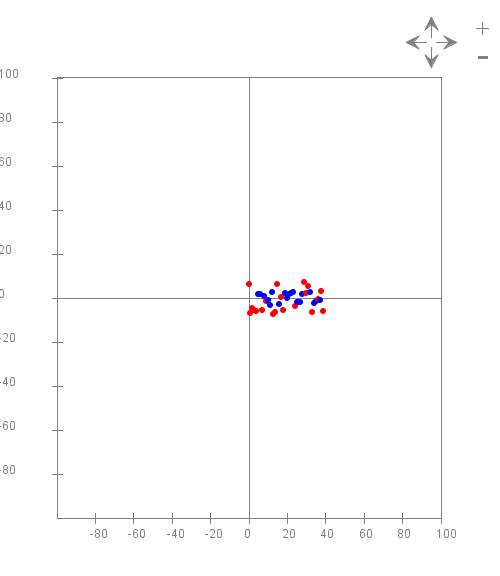
\includegraphics[scale=0.45]{exercise26}

%exercise27
\item They are easier to cluster although it is not a perfect clustering. There will blue points in the red cluster. \\
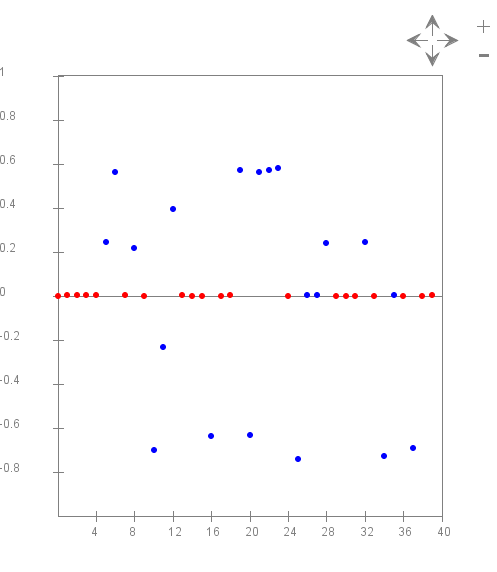
\includegraphics[scale=0.5]{exercise27}

%exercise28
\item Suppose we have data that is distributed in two concentric circles about the origin. Then, if we use the first dimension of the transformed data, we would transform the data using the following: $x^2 + y^2$. So, all data would shift to lie in the upper right quadrant, in two 'concentric' arcs. From here, it can be seen that the data is cleanly separable. 

%exercise29
\item computation of similarity: \\
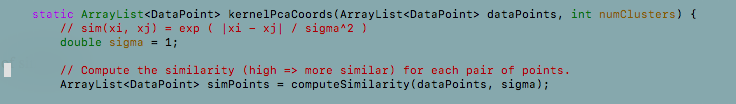
\includegraphics[scale=0.5]{exercise29}


\end{enumerate}
\end{document}